\documentclass[a4paper]{article}
\usepackage{graphicx}
\usepackage{fancyhdr}
\usepackage{geometry}
\geometry{
	a4paper,
	total={170mm,257mm},
	left=20mm,
	top=20mm,
	bottom=39mm,
}

\setlength{\headheight}{82.70538pt}

\fancypagestyle{oida}{
	\fancyhf{}
	\fancyhead[L]{\fontsize{7.5}{7.5}htl donaustadt\\ Donaustadtstraße 45\\
		1220 Wien\\~\\ Abteilung: Informationstechnologie\\ 
	Schwerpunkt: Netzwerktechnik}
	\fancyhead[R]{
\includegraphics[scale=0.45]{logo.png}}

	\fancyfoot[L]{\today}
	\fancyfoot[C]{\jobname}
	\fancyfoot[R]{Seite: \thepage}
}

\begin{document}
\pagestyle{oida}
\section*{Thema}
\par\noindent\rule{\textwidth}{0.4pt}

Laborprotokoll

\begin{figure}[h]
	
\includegraphics[scale=0.6]{meme.jpeg}
	\caption{memes klauen ist nicht ethisch}
\end{figure}

\vspace*{\fill}
Unterrichtsgegenstand:	NWT1|ZIVK

Jahrgang:	2BHIT

Name:	Stefan Fürst

Betreuer: 	ZIVK

Übungsdaten:	Datum

Abgabedatum:	Datum


\newpage
\tableofcontents

\newpage

\section{Aufgabenstellung}
Statisches Routing in einem großen Netzwerk einzeichnen, Routing Tabellen machen und durch die GUI eine Kommunikation ermöglichen.
\section{Zusammenfassung}
Tonnenweise Pfeile zeichnen und Tabellen machen und Packet Tracer UX genießen.
\newpage

\section{Vollständige Netzwerktopologie der gesamten Übung}

\begin{figure}[h]
	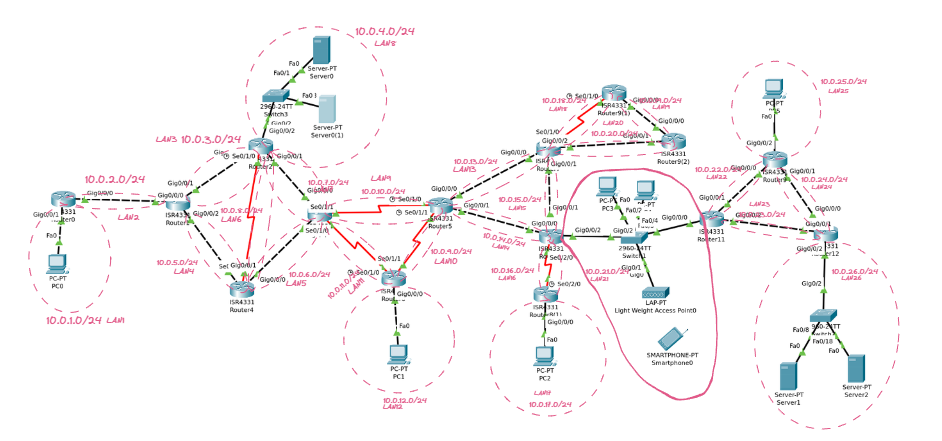
\includegraphics[scale=0.5]{topologie.png}
	\caption{Netzwerktopologie der Übung}
\end{figure}

\newpage

\section{Übungsdurchführung}

\subsection{Routing Tabellen}
\subsubsection{Pc 5 zu Server 1}



\subsection{Einstellen der Statischenn Routen in Packet Tracer mit der Gui.}

\newpage

\section{Abbildungsverzeichnis}

\listoffigures

\end{document}
